% !TEX root = thesis.tex

\chapter{Incremental construction}
\label{ch:incremental-construction}

In addition to the extrusion method presented in \refch{ch:extrusion}, an $n$-cell can also be constructed based on a set of $(n-1)$-cells known to form its complete (closed) boundary.
This kind of process is significantly more complex than extrusion.
However, unlike extrusion it permits the creation of cells of arbitrary shape.
It can also be applied cell by cell in increasing dimension, starting with the construction of isolated 0-cells first and continuing through 2-cells, 3-cells and further, allowing for the \emph{incremental construction} of objects of any dimension.

This chapter describes an operation that permits the aforementioned process to be easily applied in practice using a topological data structure.
Based on combinatorial maps (\refse{ss:ordered-topological-models}) and their fundamental operations (\refse{ss:operations-maps}), it connects the separate boundary cells together and computes the topological relationships between them, encapsulating low-level details such as the creation and deletion of individual combinatorial elements with appropriate orientations.

The chapter begins with some background on the operations and a description of the overall approach in \refse{se:incremental-approach}.
It then explains the steps needed to create the cells of each dimension in \refse{se:primitives}.
\refse{se:incremental-implementation} describes how the approach was implemented based on the Computational Geometry Algorithms Library (CGAL).
\refse{se:incremental-experiments} summarises some experiments based on this implementation, generating relatively large objects in up to 4D.
Finally, \refse{se:incremental-conclusions} concludes the chapter with the possibilities to use incremental construction to build higher-dimensional datasets.

Most of this chapter is based on the paper:
\begin{itemize}
\papericaaincrementalconstruction%
\end{itemize}

\section{Background and overall approach}
\label{se:incremental-approach}

Based on the Jordan-Brouwer separation theorem \citep{Lebesgue11,Brouwer11}, it is known that a subset of space homeomorphic to an $(n-1)$-dimensional sphere\footnote{A generalisation of the concept of a sphere in arbitrary dimensions.
A 0-sphere is the pair of points, a 1-sphere is a circle, and a 2-sphere a sphere. As opposed to disks and balls, circles and spheres are hollow.} $S^{n-1}$ in the $n$-dimensional Euclidean space $\mathbb{R}^n$ divides the space into two connected components: the \emph{interior}, which is the region bounded by the sphere, and the \emph{exterior}.
This means that the principles of boundary representation as described in \refse{ss:data-models} extend to higher dimensions, and so an $n$-cell in a cell complex can be described (and therefore constructed) based a set of $(n-1)$-cells that are known to form its complete (closed) boundary\footnote{This is true in practice.
However, there are fractal-like pathological objects where this is not the case because their interior or exterior components are not homeomorphic to disks \citep{Alexander24}.
This type of objects will certainly not be constructed using this method.}.

The \emph{incremental construction} method proposed in this chapter exploits this property by applying this process cell by cell in increasing dimension.
Isolated vertices are first constructed, which can be uniquely defined based on their coordinates.
These vertices can then be connected to form individual edges, or alternatively to form cycles of edges representing faces directly, as in most of the typical GIS approaches described in \refse{ss:formats}.
Sets of faces can be connected to form volumes, sets of volumes to form 4-cells and so on.

In a similar manner as extrusion, presented in \refch{ch:extrusion}, this \emph{incremental construction} process significantly reduces the conceptual complexity of defining and creating higher-dimensional objects.
The $(n-1)$-dimensional boundary of an $n$-cell is much easier to conceive than the original $n$-cell because it can be subdivided into multiple simpler $(n-1)$-cells, which can be individually described and constructed using the same method.

However, applying this incremental construction process using a topological data structure is not that simple, as it involves many intricate small problems: finding the topological relationships between the cells, appropriately connecting them, keeping track of multiple connected components, avoiding the creation of duplicate cells (as part of the boundary of independently-described higher-dimensional cells), changing the orientation of cells on the fly (since those that have been created separately will often have incompatible orientations), and detecting non-manifold shapes, among others.

The incremental construction operator presented in this chapter solves all of the aforementioned issues efficiently.
It is based on $n$-dimensional combinatorial maps with linear geometries and it is fully dimension-independent.
As it generates all the incidence and adjacency relationships between $(n-1)$-cells in an $n$-dimensional cell complex, it can also be used to obtain these relationships when needed, such as when multiple datasets are combined into one or when a non-topological representation is instead used (\eg\ the Simple Features-like approach shown in \refse{ss:nd-topology}).

In order to be efficient, the algorithm uses two basic techniques: (i) indexes on the lexicographically smallest vertex (\refse{se:spatial-indexing}) of certain cells, which are used in order to keep track of individual cells (which might be disconnected) and to access cells efficiently; and (ii) signature-generating traversals for specific cells \citep{Gosselin11}, which are used to efficiently compare whether two cells are equivalent by checking if it is possible to find an isomorphism $f$ that maps darts with equivalent $\beta$ relations and embedded at the same locations in space, as was shown in \refse{se:ndqueries}.

\section{Incremental construction of primitives per dimension}
\label{se:primitives}

The idea of the incremental construction algorithm is to construct cells individually, using lower-dimensional cells that have already been constructed in order to describe part of the boundary of a higher-dimensional cell.
In terms of the darts of a combinatorial map, this sometimes implies the reuse of existing darts, and sometimes the creation of new ones which are connected to the existing ones.
There is however no strict requirement that the cells are created in strictly increasing dimension, and so new cells can be easily added to an existing cell complex.

Due to the need to embed 0-cells into a point in space, as well as the oriented nature of a combinatorial map, the incremental construction method is different for 0-, 1- and 2-cells.
3-cells and those of higher dimensions follow the same procedure.
These are therefore described separately below, using as an example the creation of the pair of adjacent tetrahedra shown in \reffig{fig:2tetra}.
\marginpar{
\captionsetup{type=figure}
\centering
\subfloat[]{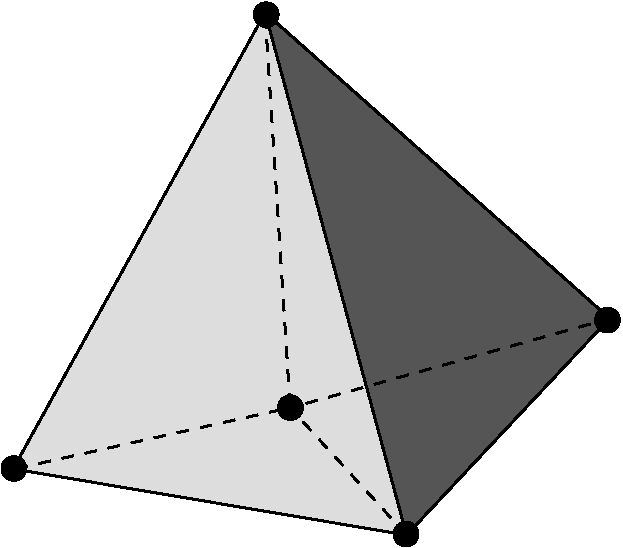
\includegraphics[width=\marginparwidth]{figs/2tetra}} \\
\subfloat[]{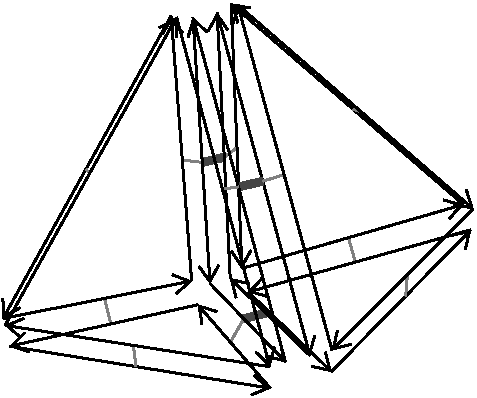
\includegraphics[width=\marginparwidth]{figs/2tetra-map}}
\caption[Two adjacent tetrahedra as a combinatorial map]{(a) Two adjacent tetrahedra and (b) their representation as a combinatorial map.}
\label{fig:2tetra}
}

\subsection{Vertices (0-cells)}
\label{ss:incremental-vertices}

The aim of the process of 0-cell construction is to create an isolated dart and an associated point embedding structure for every 0-cell, while avoiding having duplicate embedding structures having the same point coordinates.
By making point embeddings unique---as defined by their coordinates---, they can be used to compare 0-cells without checking an entire tuple of coordinates.
Moreover, by maintaining an index of all point embeddings and links from every point embedding to a dart there, it is possible to use this index to access the combinatorial structure at that point.
In this manner, it is possible to find either an already free dart that can be reused, or a non-free dart that is part of a larger combinatorial structure, which can be copied and its copy then used.

Thus, calling a function $\texttt{make\_0\_cell(}x_0, \ldots, x_n\texttt{)}$ with the coordinates $x_0, \ldots, x_n$ describing an $n$-dimensional point, should use the index of 0-cells to return an existing dart embedded at that location (using an existing point embedding) if one exists, or a new dart embedded at that location (using a new point embedding) otherwise.
In the latter case, the new point embedding and its associated dart should be added to the index.
The result of calling this function for all the points in \reffig{fig:2tetra} is shown in \reffig{fig:reconstruction-0}.
Note that the result is identical whether the function is called once for every unique vertex, or multiple times (\eg\ once for every vertex in every face or volume).
\marginpar{
\captionsetup{type=figure}
\centering
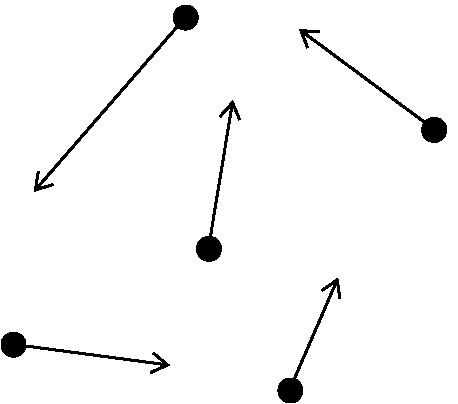
\includegraphics[width=\marginparwidth]{figs/reconstruction-0}
\caption[Constructing the 0-cells of \reffig{fig:2tetra}]{Constructing the 0-cells of \reffig{fig:2tetra} consists of creating exactly one dart embedded at each point.
These darts are isolated (\ie\ not linked by any $\beta$ relations to other darts).
The direction of the arrows shown here is arbitrary.}
\label{fig:reconstruction-0}
}

\subsection{Edges (1-cells)}
\label{ss:incremental-edges}

Generally, it is best to skip the generation of 1-cells and proceed directly to the creation of 2-cells from sequences of points.
In order to represent a single edge in a combinatorial map not one but \emph{two} darts are required: one embedded at each of the two vertices bounding the edge.
More precisely, taking into account the (arbitrary) orientation defined for the edge, the dart embedded at the \emph{origin} of the edge is connected to the \emph{destination} by $\beta_1$, and the destination is connected to the origin by $\beta_1^{-1}$.
Having two darts per edge is not a major problem, but it often creates unnecessary darts and unnecessary connections between them.
If a single face that uses all the edges is then created, half of the darts lose their original purpose (\ie\ to store a connection to their point embeddings) and might be eliminated, which is accompanied with having to reset their $\beta$ relationships.

In addition, as shown in \refse{ss:formats}, polygons can be easily described as an ordered sequence of vertices connected by implicit line segments.
Therefore, incrementally constructing $1$-cells often brings no efficiency gains or practical benefits, and so it is normally best to skip dimension one, constructing 2D facets from a sequence of 0D points, 3D volumes from their 2D faces, 4-cells from their 3-cell faces, and so on.

However, there is an exception to this rule.
Linear objects sometimes do need to be explicitly represented, either as single line segments or as polygonal lines.
In this case, it is possible to simply follow the process described for 2-cells below, omitting sewing the last dart of the line segment or polygonal line to the first dart (and vice versa), and appropriately using the 1-cells index to find if a given 1-cell already exists, or otherwise to index the newly created 1-cell or 1-cells (in the case of a polygonal line).

\subsection{Faces (2-cells)}
\label{ss:incremental-faces}

Starting from the unique 0-cells obtained from the procedure presented in \refse{ss:incremental-vertices}, in order to create a 2-cell from a sequence of 0-cells, three general steps are needed:
\begin{figure*}[tb]
\centering
\subfloat[]{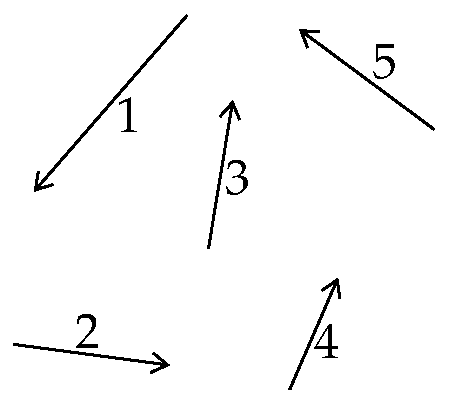
\includegraphics[width=0.22\linewidth]{figs/reconstruction-2}} \quad
\subfloat[]{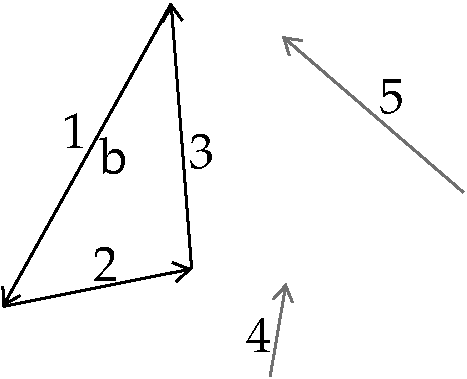
\includegraphics[width=0.22\linewidth]{figs/reconstruction-2-a}\label{subfig:reconstruction-2-a}} \quad
\subfloat[]{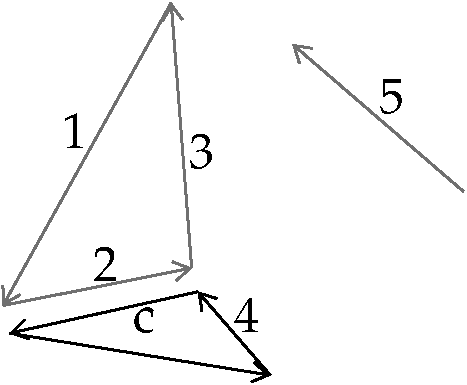
\includegraphics[width=0.22\linewidth]{figs/reconstruction-2-b}\label{subfig:reconstruction-2-b}} \quad
\subfloat[]{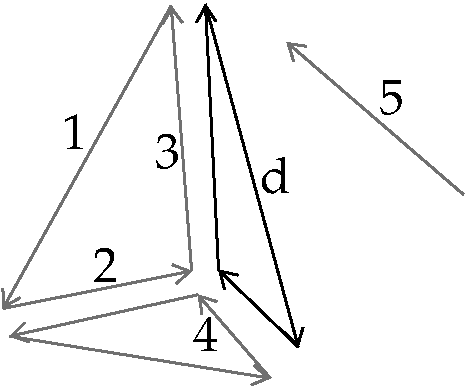
\includegraphics[width=0.22\linewidth]{figs/reconstruction-2-c}}\\
\subfloat[]{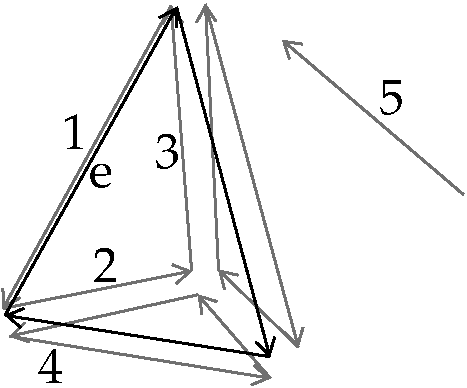
\includegraphics[width=0.22\linewidth]{figs/reconstruction-2-d}} \quad
\subfloat[]{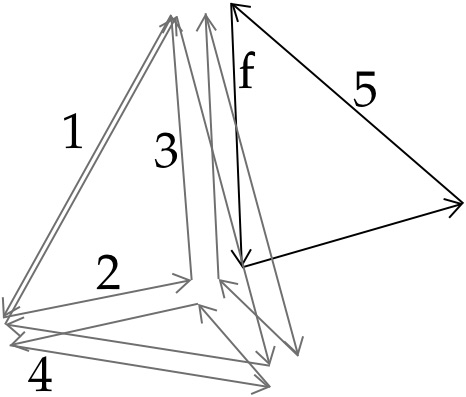
\includegraphics[width=0.22\linewidth]{figs/reconstruction-2-e}}\quad
\subfloat[]{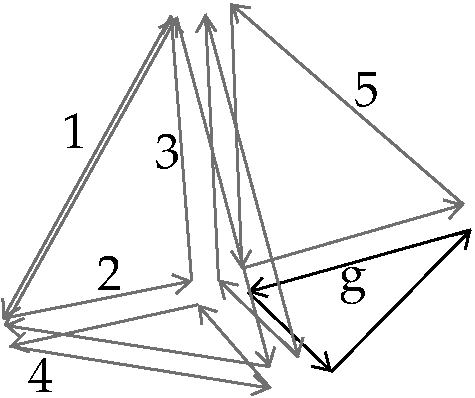
\includegraphics[width=0.22\linewidth]{figs/reconstruction-2-f}} \quad
\subfloat[]{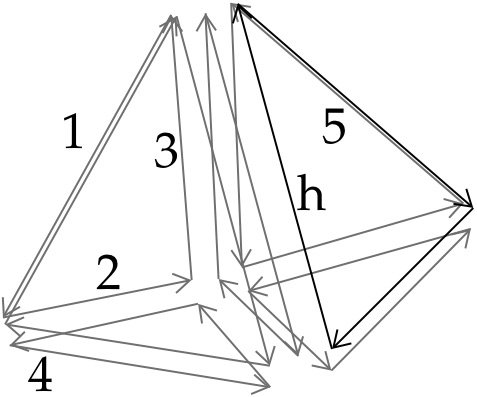
\includegraphics[width=0.22\linewidth]{figs/reconstruction-2-g}\label{subfig:reconstruction-2-g}}\\
\caption[Constructing the 2-cells of \reffig{fig:2tetra}]{The construction of the 2-cells of \reffig{fig:2tetra}. (a)~Initial configuration: one dart per vertex. (b)~After $b=\texttt{make\_2\_cell(}1,2,3\texttt{)}$. (c)~After $c=\texttt{make\_2\_cell(}2,4,3\texttt{)}$. (d)~After $d=\texttt{make\_2\_cell(}1,4,3\texttt{)}$. (e)~After $e=\texttt{make\_2\_cell(}1,4,2\texttt{)}$. (f)~After $f=\texttt{make\_2\_cell(}1,3,5\texttt{)}$. (g)~After $g=\texttt{make\_2\_cell(}5,3,4\texttt{)}$. (h)~Final result, after $h=\texttt{make\_2\_cell(}4,5,1\texttt{)}$.}
\label{fig:reconstruction-2}
\end{figure*}

\begin{enumerate}

\item
The procedure first checks if the 2-cell that is being requested already exists\footnote{This test can also be done at the end of the process, which makes it possible to use the easy cell comparison method described in \refse{se:ndqueries}.
In that case, the newly created cells (in the form of darts) that are found to be redundant should be deleted and removed from the indices.}.
Just as in the creation of 0-cells, a 2-cell being requested might have already been created, either independently or as part of a 3-cell.
This can be easily checked using the index of 2-cells with the lexicographically smallest vertex of the 0-cells being passed, and finding if from a dart starting at the lexicographically smallest vertex and following the $\beta_1$ or $\beta_1^{-1}$ relations, one passes through the same point embeddings as those passed to this construction method.

\item
Each of these 0-cells might be a $1$-free dart $d$ (\ie\ $\beta_1(d) = \emptyset$) and no dart linked by $\beta_1$ to it \ie\ $\beta_1^{-1}(d) = \emptyset$, or if $\beta_1^{-1}$ is not stored, $\nexists d^\prime \mid \beta_1(d^\prime) = d$, \emph{in which case it can be used directly}, such as in \reffig{subfig:reconstruction-2-a}.
It can also be a non $1$-free dart or one that has a dart linked by $\beta_1$ to it, which means that it is used as part of a $1$-cell (and possibly other higher dimensional cells).

The darts that are already used as part of $1$-cells are more difficult to handle, as they \emph{can be reused only when the 1-cell they are part of is also part of the boundary of the $2$-cell that will be constructed using this method}.
This needs to be tested in both possible orientations for the sequence of 0-cells, possibly resulting in the reversal of the orientation of some 1-cells.
If a given dart \emph{cannot be reused} (because it is part of a 1-cell that is not part of the 2-cell to be created), a copy of it has to be created.
The result of this step is thus a list that contains for every 0-cell a reusable or a newly created dart.

\item
The darts obtained in the previous step are 1-sewn sequentially (using $\beta_1$ and $\beta_1^{-1}$), and the last is 1-sewn to the first, forming a closed cycle.
During these sewing operations, the function checks whether every newly created edge (consisting of one dart) is present in the 1-cells index.
If a given 1-cell is already there, the new edge's dart is linked to its edge embedding structure.
If a 1-cell is not there, the edge is added to the index, a new edge embedding is created, and the edge's dart is linked to it.
Finally, the newly created 2-cell is then added to the index of 2-cells.

In order to verify that the 2-cell being generated is a quasi-manifold, it is useful to assert that all darts that are $1$-free and have a $\beta_1^{-1}$ set to $\emptyset$ at the beginning of this third step, \ie\ those that were not copied, should continue to be $1$-free and have a $\beta_1^{-1}$ set to $\emptyset$ until they are sewn.
This ensures that a vertex is not used twice within the same face, and as such, that the 2-cell is a quasi-manifold.

\end{enumerate}

\reffig{fig:reconstruction-2} shows the incremental construction procedure for all the 2-cells of \reffig{fig:2tetra}, which consists of 7 2-cells and is thus obtained by 7 calls to the \texttt{make\_2\_cell} method.

\subsection{Volumes (3-cells) and higher}
\label{ss:incremental-volumes}

The method to create $i$-cells from their $(i-1)$-cell boundaries is identical for all $i > 2$, allowing for a fully dimension-independent function to be created.
This function consists of four general steps:

\begin{enumerate}

\item
First of all, the procedure checks whether each $(i-1)$-cell that is passed is $(i-1)$-free or not.
If it is $(i-1)$-free, it is reused as part of the $i$-cell, such as in \reffig{subfig:reconstruction-3-a}.
If it is not $(i-1)$-free, then it is already part of a different $i$-cell, so a copy of it is made \emph{with reverse orientation}, as shown in \reffig{subfig:reconstruction-3-b}.
This copy can then be used for the construction of the $i$-cell.

For a given dart $d$ that is known to be part of the $(i-1)$-cell, this copy can be made by taking all the darts in the orbit $C = \langle \beta_1, \ldots, \beta_{i-2} \rangle (d)$, creating a new set of darts $C^\prime$ to contain the copied darts and inserting a new dart in $C^\prime$ for every dart in $C$.
Using a function $f : C \rightarrow C^\prime$ that maps a dart in $C$ to its corresponding dart in $C^\prime$, for every dart $c \in C$ the $\beta_1$ relations are set as $\beta_1^{-1}\left(f\left(c\right)\right) = f\left(\beta_1\left(c\right)\right)$ and $\beta_1\left(f\left(c\right)\right) = f\left(\beta_1^{-1}\left(c\right)\right)$. For the ones of higher dimensions, they are set such that $\forall 2 \leq j \leq i-2$, $\beta_j\left(f\left(c\right)\right) = f\left(\beta_j\left(c\right)\right)$.

Note that the combinatorial structures are copied with reversed orientation, as this ensures that the two (old and new) can be directly $i$-sewn together, if necessary.

\item
A temporary \emph{ridge index} of the $i$-cell is built, containing all the $(i-2)$-cells on the boundary of all $(i-1)$-cells that have been passed to the construction method---not all the $(i-1)$-cells in the cell complex---using their lexicographically smallest vertices, such that their index entries link to a usable dart in the $(i-2)$-cell with a point embedding at the lexicographically smallest vertex.
This dart should be one that is $(i-1)$-free, either because it was already free as part of the combinatorial structure of the passed $(i-1)$-cells, or because it is a copy (with reversed orientation) of one that was not $(i-1)$-free.

\item
Using the ridge index, $(i-1)$-cells (\ie\ facets) are $(i-1)$-sewn along their common $(i-2)$-cell boundaries (\ie\ ridges).
For this, for every $(i-2)$-cell on the boundary of an $(i-1)$-cell passed to the function, exactly one matching $(i-2)$-cell should be found in the index, which should be equivalent as compared using the method described in \refse{se:ndqueries} and might be of the same or opposite orientation (but not the same $(i-1)$-cell).
This criterion ensures that a quasi-$(i-1)$-manifold will be constructed.

If the two $(i-1)$-cells are sewable along their common $(i-2)$-cell boundaries, \ie\ they have compatible orientations, they are directly sewn together.
Otherwise, the orientation of the entire connected component of either of the two $(i-1)$-cells should be reversed.
If the two $(i-1)$-cells have incompatible orientations but are part of the same connected component, the cell that is being requested is unorientable, and thus cannot be represented using combinatorial maps.
As long as it forms a quasi-manifold it can however be represented using generalised maps.

\item
Using the index of $i$-cells, the newly constructed $i$-cell is compared to others to check if it had already been created, which is also done using the lexicographically smallest vertex of the cell.
If an equivalent $i$-cell (with the same or opposite orientation) is found, the function deletes the newly created darts of the cell and instead returns the existing $i$-cell.
If an equivalent $i$-cell is not found, the newly created cell is added to the index and returned.

\end{enumerate}

\reffig{fig:reconstruction-3} shows the incremental construction procedure for the two 3-cells of \reffig{fig:2tetra}.
\marginpar{
\captionsetup{type=figure}
\centering
\subfloat[]{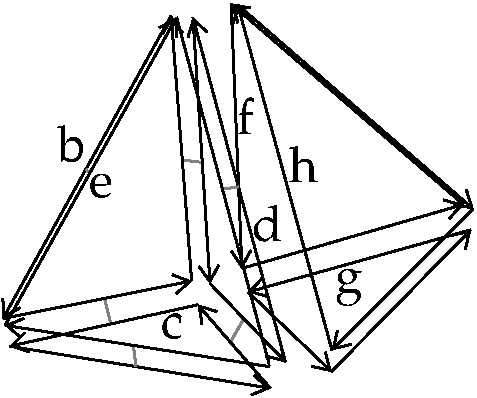
\includegraphics[width=\marginparwidth]{figs/reconstruction-3-a}\label{subfig:reconstruction-3-a}} \\
\subfloat[]{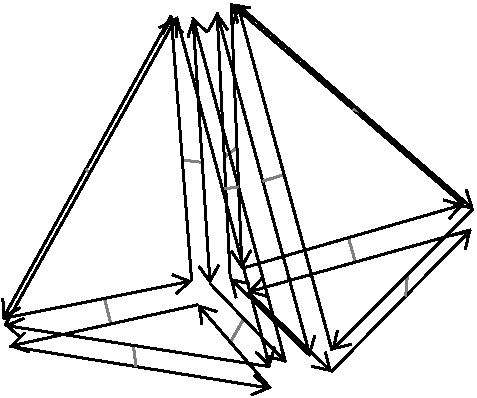
\includegraphics[width=\marginparwidth]{figs/reconstruction-3-b}\label{subfig:reconstruction-3-b}}
\caption[Constructing the 3-cells of \reffig{fig:2tetra}]{The construction of the 3-cells of \reffig{fig:2tetra}. (a)~After $\texttt{make\_3\_cell(}b,c,d,e\texttt{)}$. (b)~Final result, after $\texttt{make\_3\_cell(}e,f,g,h\texttt{)}$.}
\label{fig:reconstruction-3}
}

\section{Implementation and complexity analysis}
\label{se:incremental-implementation}

The incremental construction algorithm has been implemented in C++11 and made available under the open source MIT licence at \url{https://github.com/kenohori/lcc-tools}.
As the extrusion related code (\refse{se:extrusion-implementation}), it requires and builds upon the CGAL packages Combinatorial Maps and Linear Cell Complex, among others.
% The first package provides data structures and algorithms to store and to efficiently iterate over the darts of a combinatorial map, and the second links the 0-embeddings to other CGAL types in order to store the geometry of a model.

For this prototype implementation, the lexicographically smallest vertex indices were implemented as C++ Standard Library \texttt{maps}\footnote{The exact implementation depends on the library that is used, but normally they are red-black trees.} for every dimension, using point embeddings as keys and \texttt{lists} of darts as values.
Each dart in a \texttt{list} represents a separate cell (of the dimension of the index) that has that point as its lexicographically smallest.
A custom comparison function is used so that the points are internally sorted in lexicographical order.
As a \texttt{map} has $O(\log n)$ search, insertion and deletion times and $O(n)$ space \citep[\S{}23.4]{ISO14882:2015}, all of these operations can be performed efficiently.

If a truly incremental construction approach is followed, creating all $i$-cells before proceeding to the $(i+1)$-cells, it is not necessary to maintain indices for all the cells of all dimensions at the same time.
The only ones that are needed are those for: all $i$- and $(i-1)$-cells, as well as a temporary index for the $(i-2)$-cells on the boundary of the $(i-1)$-cells for one given $i$-cell.
This means that only three indexes need to be kept at a given time.

Most of these can be built incrementally, adding new cells as they are created in $O(\log c)$, with $c$ the number of cells of that dimension, assuming that the smallest vertex and a dart embedded there are kept during its construction.
The complexity of building any index of cells of any dimension is thus $O(c \log c)$ and it uses $O(c)$ space.

Checking whether a given cell already exists in the cell complex is more complex.
Finding a list of cells that have a certain smallest vertex is done in $O(\log c)$.
Theoretically, all existing cells in the complex could have the same smallest vertex, leading to up to $c$ quadratic time cell-to-cell comparisons just to find whether one cell exists.
However, every dart is only part of \emph{a single} cell of any given dimension\footnote{This is true for the type of combinatorial maps that are handled here, but not in the general case.}, so while every dart could conceivably be a starting point for the comparison, a single dart cannot be used as a starting point in more than one comparison, and thus a maximum of $d_{\mathrm{complex}}$ identity comparisons will be made for \emph{all} cells, with $d_{\mathrm{complex}}$ being the total number of darts in the cell complex.
From these $d_{\mathrm{complex}}$ darts, two identity comparisons are started, one assuming that the two cells (new and existing) have the same orientation, and one assuming opposite orientations.
Each of these involves a number of dart-to-dart comparisons in the canonical representations that \emph{cannot} be higher than the number of darts in the smallest of the two cells.
The number of darts in the existing cell is unknown, but starting from the number of darts in the newly created cell ($d_{\mathrm{cell}}$), it is safe to say that no more than $d_{\mathrm{cell}}$ dart-to-dart comparisons will be made in each identity test, leading to a worst-case time complexity of $O(d_{\mathrm{complex}} d_{\mathrm{cell}})$.
Note that this is similar to an isomorphism test starting at every dart of the complex.

Finally, creating an $i$-cell from a set of $(i-1)$-cells on its boundary is more expensive, since the $(i-2)$-cell (ridge) index needs to be computed for every $i$-cell.
Following the same reasoning as above, it can be created in $O(r \log r)$ with $r$ the number of ridges in the $i$-cell, and uses $O(r)$ space.
Checking whether a single ridge has a corresponding match in the index is done in $O(d_{\mathrm{cell}} d_{\mathrm{ridge}})$, with $d_{\mathrm{cell}}$ the number of darts in the $i$-cell and $d_{\mathrm{ridge}}$ the number of darts in the ridge to be tested.
Since this is done for all the ridges in an $n$-cell, the total complexity of this step, which dominates the running time of the algorithm, is

\begin{equation*}
\displaystyle\sum_{\mathrm{ridges}} O(d_{\mathrm{cell}} d_{\mathrm{ridge}}) = O(d_{\mathrm{cell}}^{2}).
\end{equation*}

The analyses given above give an indication of the computational and space complexity of the incremental algorithm as a whole.
However, it is worth noting that in realistic cases the algorithm fares far better than in these worst-case scenarios: the number of cells that have a certain smallest vertex is normally far lower than the total number of cells in the complex, most of their darts are not embedded at the smallest vertex, and from these darts most identity comparisons will fail long before reaching the end of their canonical representation.

Finally, one more nuance can affect the performance of this approach.
When two connected components of darts with incompatible orientations have to be joined, the orientation of one of these has to be reversed.
This is easily done by obtaining all the connected darts of one of the connected components, preferably the one that is expected to be smaller, and reversing their orientation 2-cell by 2-cell.
Every dart $d$ in a 2-cell is then $1$-sewn to the previous dart in the polygonal curve of the 2-cell (\ie\ $\beta_{1}^{-1}(d)$).
A group of $n$ darts can thus have its orientation reversed in $O(n)$ time.
This is not a problem in practice since GIS datasets generally store nearby objects close together, but if a cell complex is incrementally constructed in the worst possible way, \ie\ creating as many disconnected groups as possible, this could have to be repeated for \emph{every} cell of every dimension, creating a very inefficient process.

\section{Experiments}
\label{se:incremental-experiments}

\subsection*{Simple comparisons with valid primitives}

The CGAL Linear Cell Complex package provides functions to generate a series of primitives (line segments, triangles, quadrangles, tetrahedra and hexahedra) which are known to be created with correct geometry and topology, and can then be sewn together to generate more complex models.
Models constructed in this manner were thus created independently and compared to those incrementally constructed using the method presented in this chapter.
By using the approach shown in \refse{se:ndqueries}, it was possible to validate that they were equivalent.

\subsection*{A tesseract}

In order to present an example in more than three dimensions, a tesseract was also incrementally constructed using the approach presented in this chapter, which is shown in \reffig{fig:tesseract-darts}.
A tesseract is a 4-cell bounded by 8 cubical 3-cells, each of which is bounded by 6 square 2-cells.
It thus consists of one 4-cell, 8 3-cells, 24 2-cells, 32 1-cells and 16 0-cells.
\marginpar{
\captionsetup{type=figure}
\centering
\subfloat[]{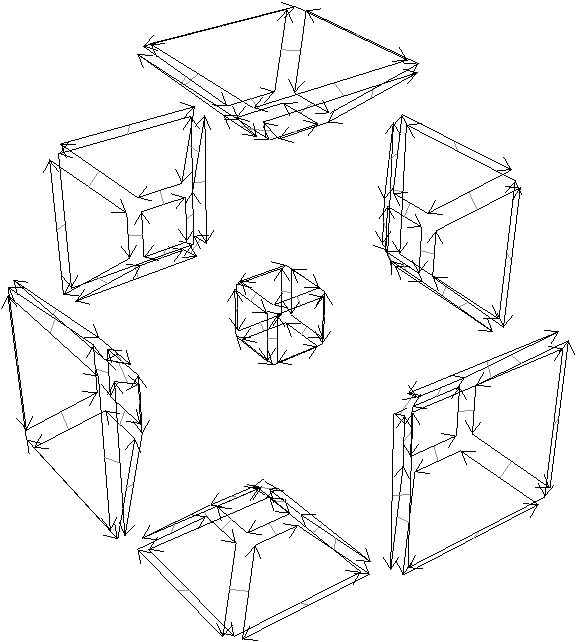
\includegraphics[width=\marginparwidth]{figs/tesseract2}} \\
\subfloat[]{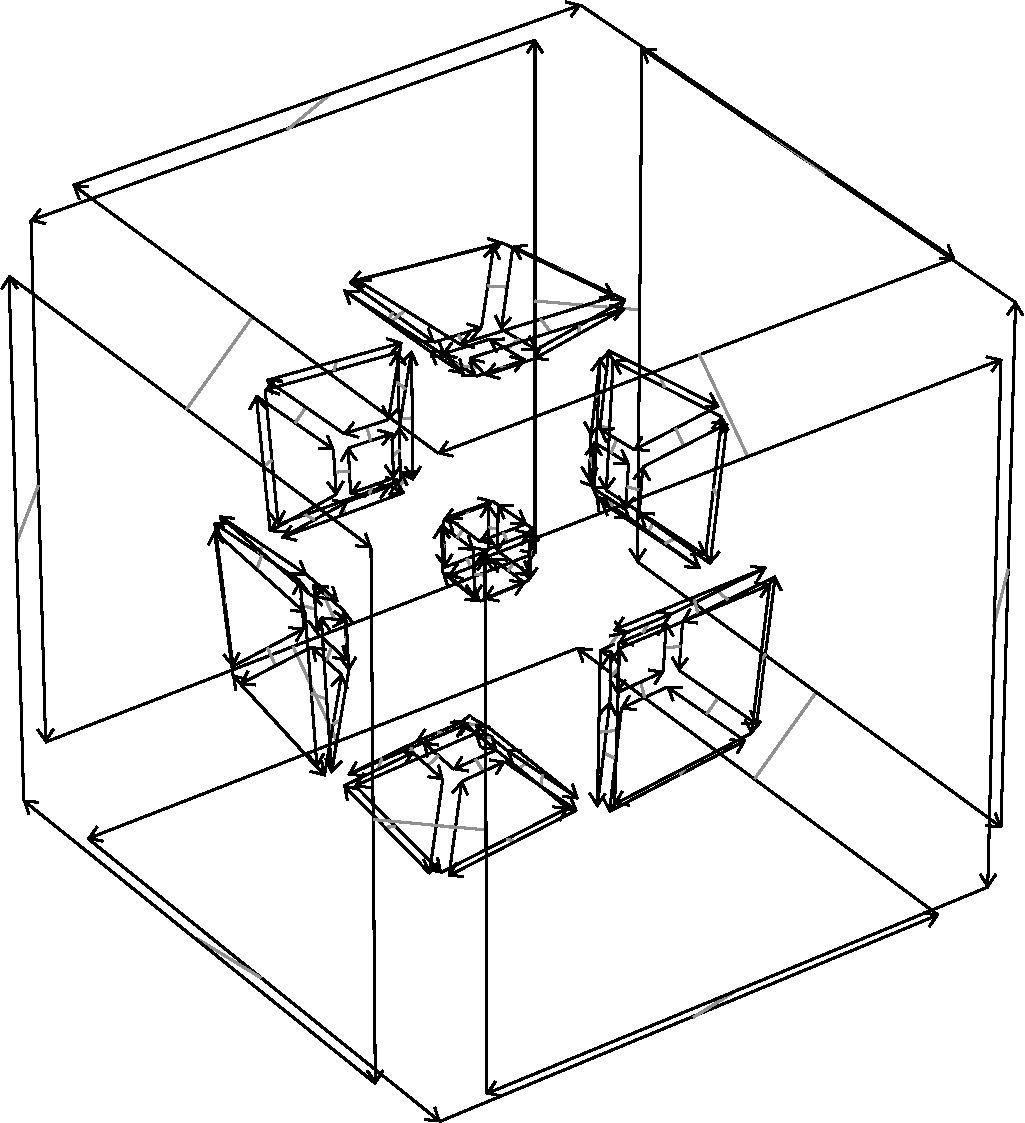
\includegraphics[width=\marginparwidth]{figs/tesseract3}} \\
\subfloat[]{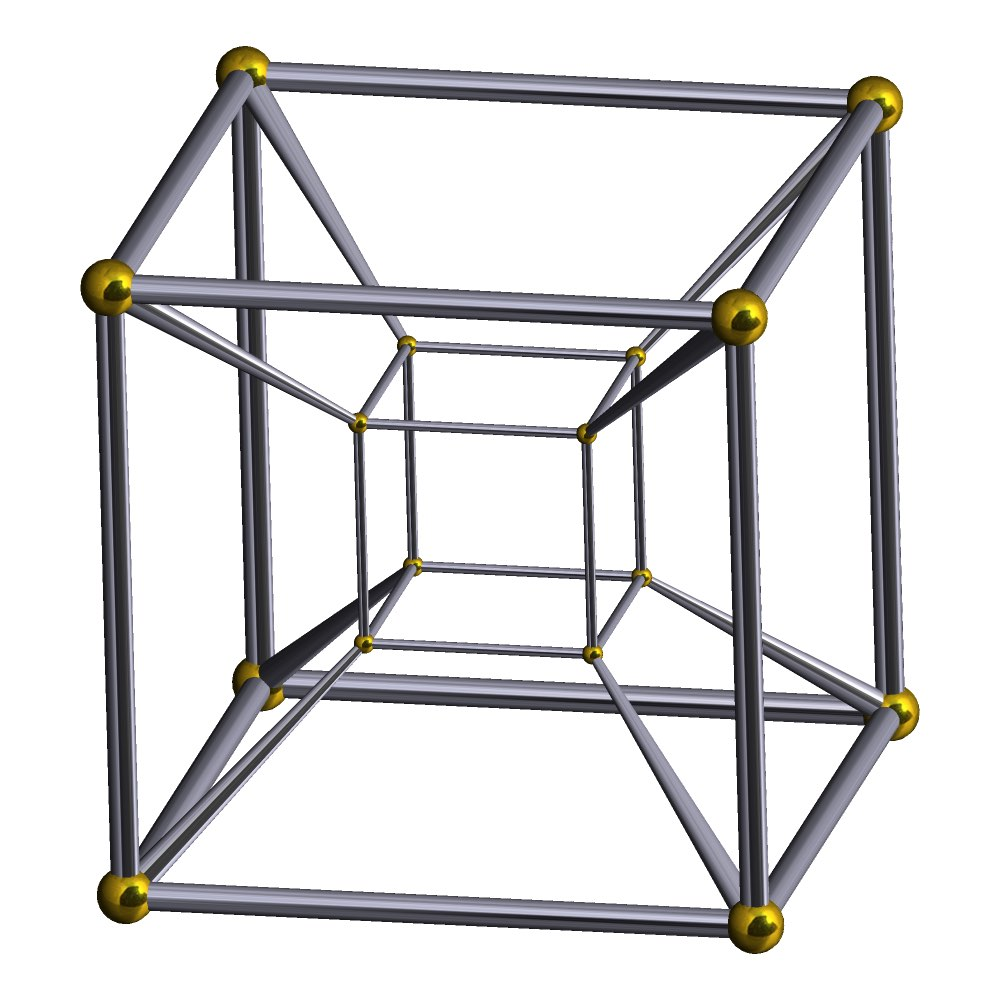
\includegraphics[width=\marginparwidth]{figs/tesseract}}
\caption[A tesseract as a combinatorial map]{A tesseract as a combinatorial map: (a) the darts of its 7 inner cubes, (b) the darts of its 8 cubes, and (c) all of its darts shown together.}
\label{fig:tesseract-darts}
}

Using the approach presented here, an empty 0-cell index is first created.
Then, the 16 vertices of the tesseract, each vertex $p_{i}$ being described by a tuple of coordinates $(x_{i},y_{i},z_{i},w_{i})$, were created as $p_{i}=\texttt{make\_0\_cell(}x_{i},y_{i},z_{i},w_{i}\texttt{)}$, which returns a unique dart embedded at each location that is also added to the 0-cell index.
At this point, the algorithm has built an unconnected cell complex consisting solely of 16 completely free darts.

An empty index of 2-cells is then created.
Each of the tesseract's 24 square facets are then built based on their vertices as $f_{i}=\texttt{make\_2\_cell(}p_{j},p_{k},p_{l},p_{m}\texttt{)}$, which 1-sews (copies of) these darts in a loop and returns the dart embedded at the smallest vertex of the facet.
These are added to the index of 2-cells.
Since every vertex is used in 6 different 2-cells, each dart would be copied 5 times.
The cell complex at this point thus consists of 24 disconnected groups of 4 darts each.

Next, an empty index of 3-cells is created and the index of 0-cells can be deleted.
For each of the 8 cubical 3-cells, a function call of the form $v_{i}=\texttt{make\_3\_cell(}f_{j},f_{k},f_{l},f_{m},f_{n},f_{o}\texttt{)}$ is made.
At this point, an index of the 1D ridges of each face is built, which is used to find the 12 pairs of corresponding ridges that are then be 2-sewn together.
When a 3-cell is created, it is added to the index.
Since every face bounds two 3-cells, each dart is duplicated once again, resulting in a cell complex of 8 disconnected groups of 24 darts each.

Finally, the tesseract is created with the function $t=\texttt{make\_4\_cell(}v_{1},v_{2},\dots,v_{8}\texttt{)}$.
This can use the index of 2-cells to find the 24 corresponding pairs of facets that are then 3-sewn to generate the final cell complex.

The validity of this object was tested by checking whether it formed a valid combinatorial map, testing whether each cube was identical to a cube created with the Linear Cell Complex package, and manually verified the $\beta$ links of its 192 darts.

\subsection*{2D+scale data}

In order to test the incremental construction algorithm and its applicability to data incorporating non-spatial characteristics, a few 2D+scale datasets from \citet{Meijers11} using ATKIS data\footnote{\url{http://www.bkg.bund.de/nn_147094/SharedDocs/Download/Barrierefreie-Textversionen/EN-InfoMaterial/EN-Text-Vector-Data.html}}, were also incrementally constructed.
As shown in \reffig{fig:utm}, these datasets model the generalisation of a planar partition as a set of stacked prisms.
Both of the simple datasets of this figure were created successfully in under a second.
\marginpar{
\captionsetup{type=figure}
\centering
\subfloat[]{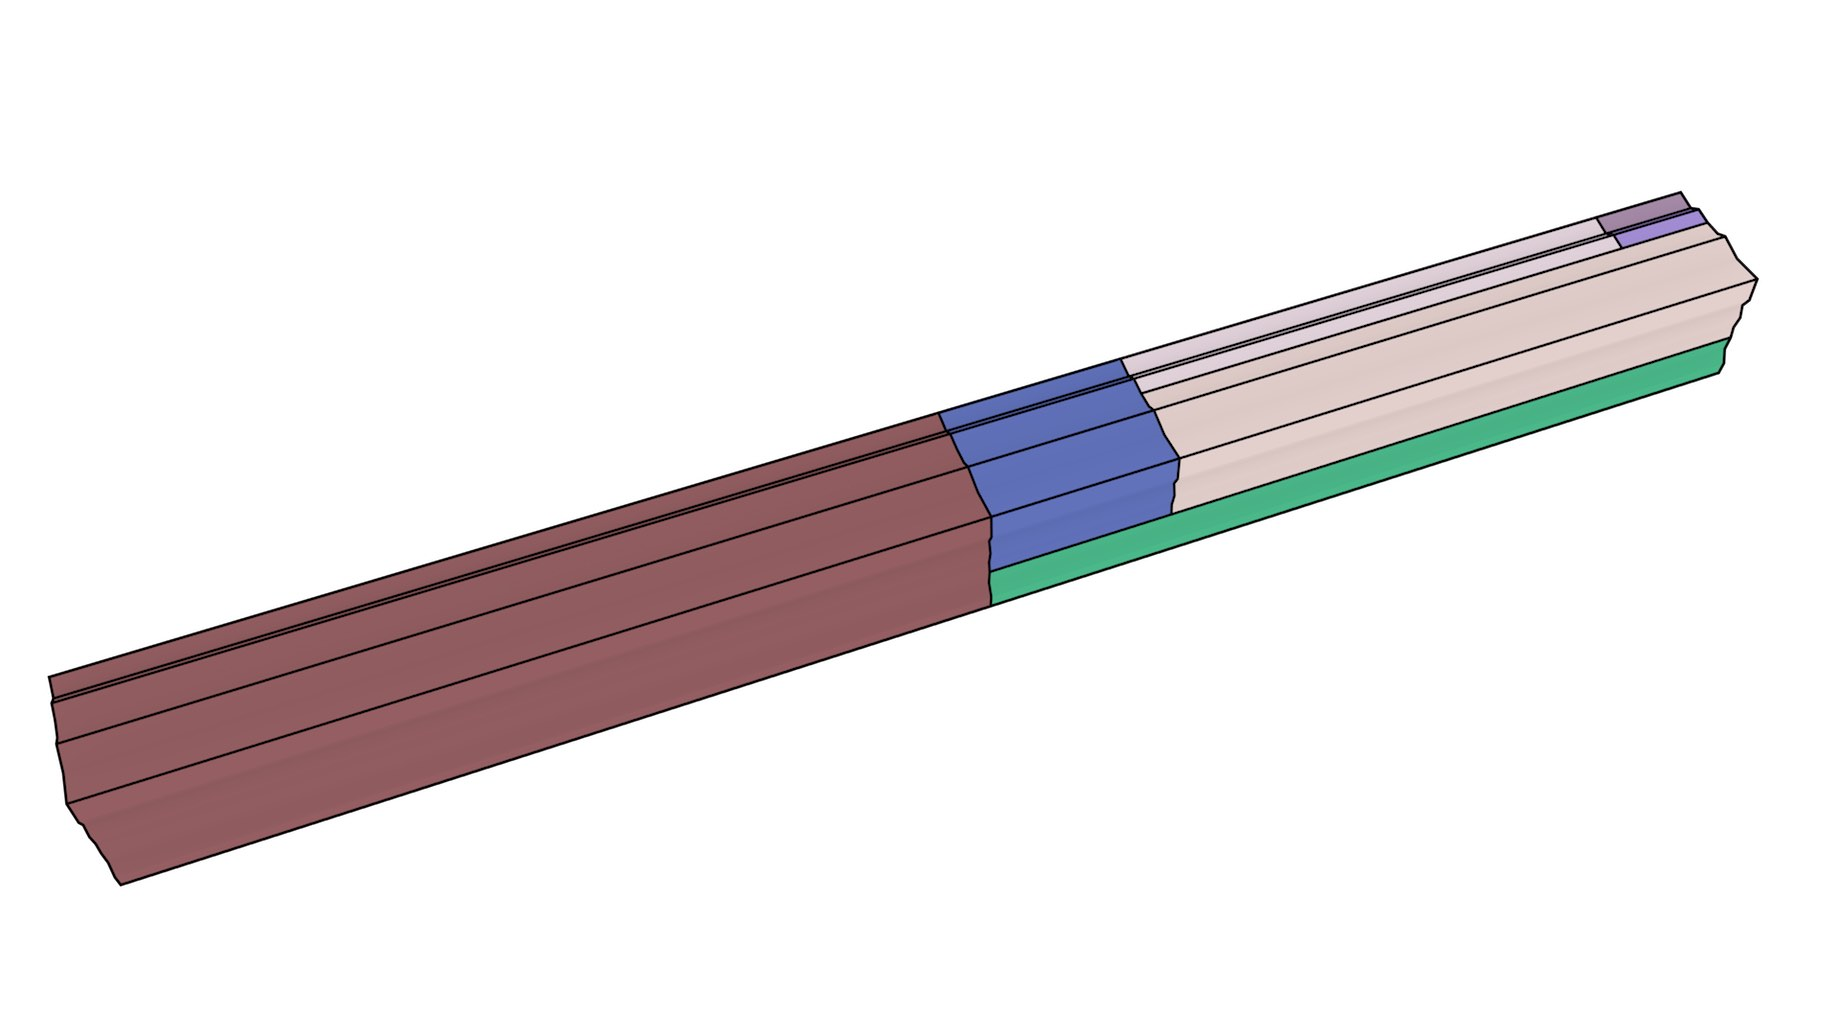
\includegraphics[width=\marginparwidth]{figs/utm}} \\
\subfloat[]{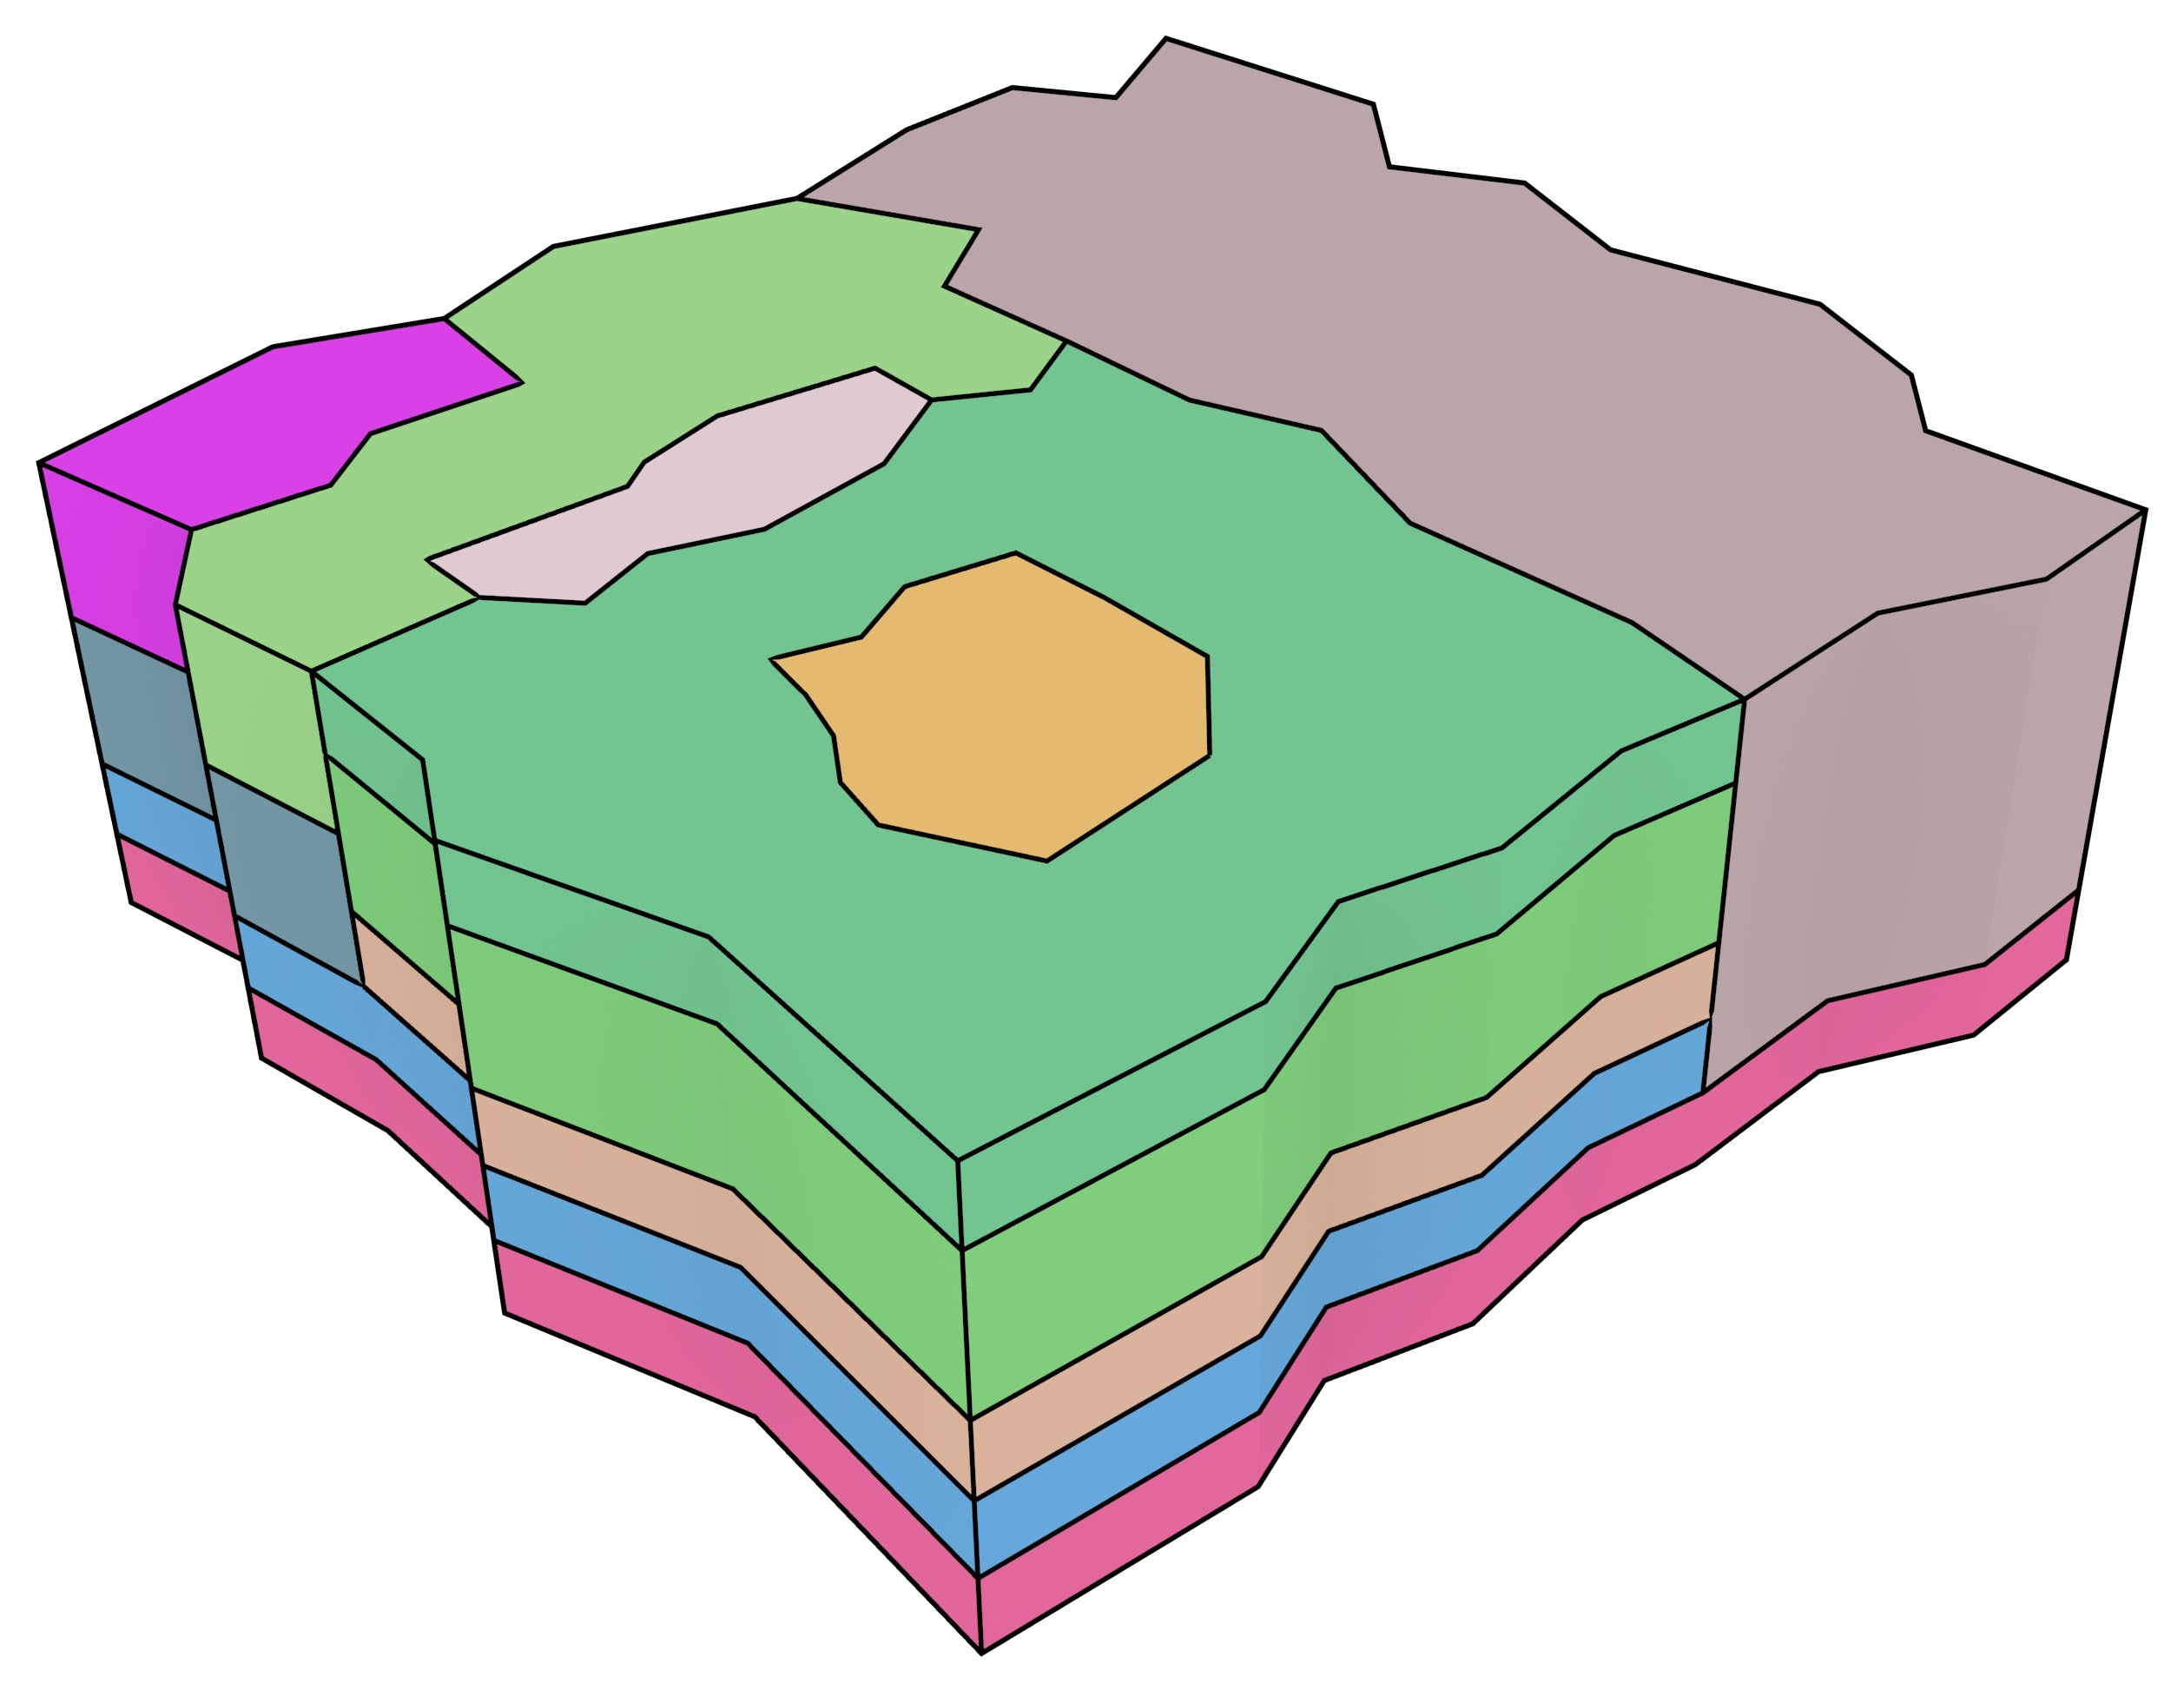
\includegraphics[width=\marginparwidth]{figs/utm2}}
\caption[Simple 2D+scale datasets]{Simple 2D+scale datasets from \citet{Meijers11}, which represent the generalisation of a planar partition by merging areas.
The dataset shown in (a) has realistic scale intervals such that the generalisation operations are performed at scales that depend on the area of a polygon, while the dataset in (b) uses equally spaced generalisation operations.}
\label{fig:utm}
}

A larger dataset, shown in \reffig{fig:atkis} and consisting of 698 polyhedra with a total of 457 185 faces, was used as a benchmark to test the performance of the algorithm.
This dataset was processed without errors in roughly 30 minutes, including validation tests to ensure that every face created was a valid combinatorial map and that the faces of a volume formed a closed quasi-manifold.
\begin{figure}[bp]
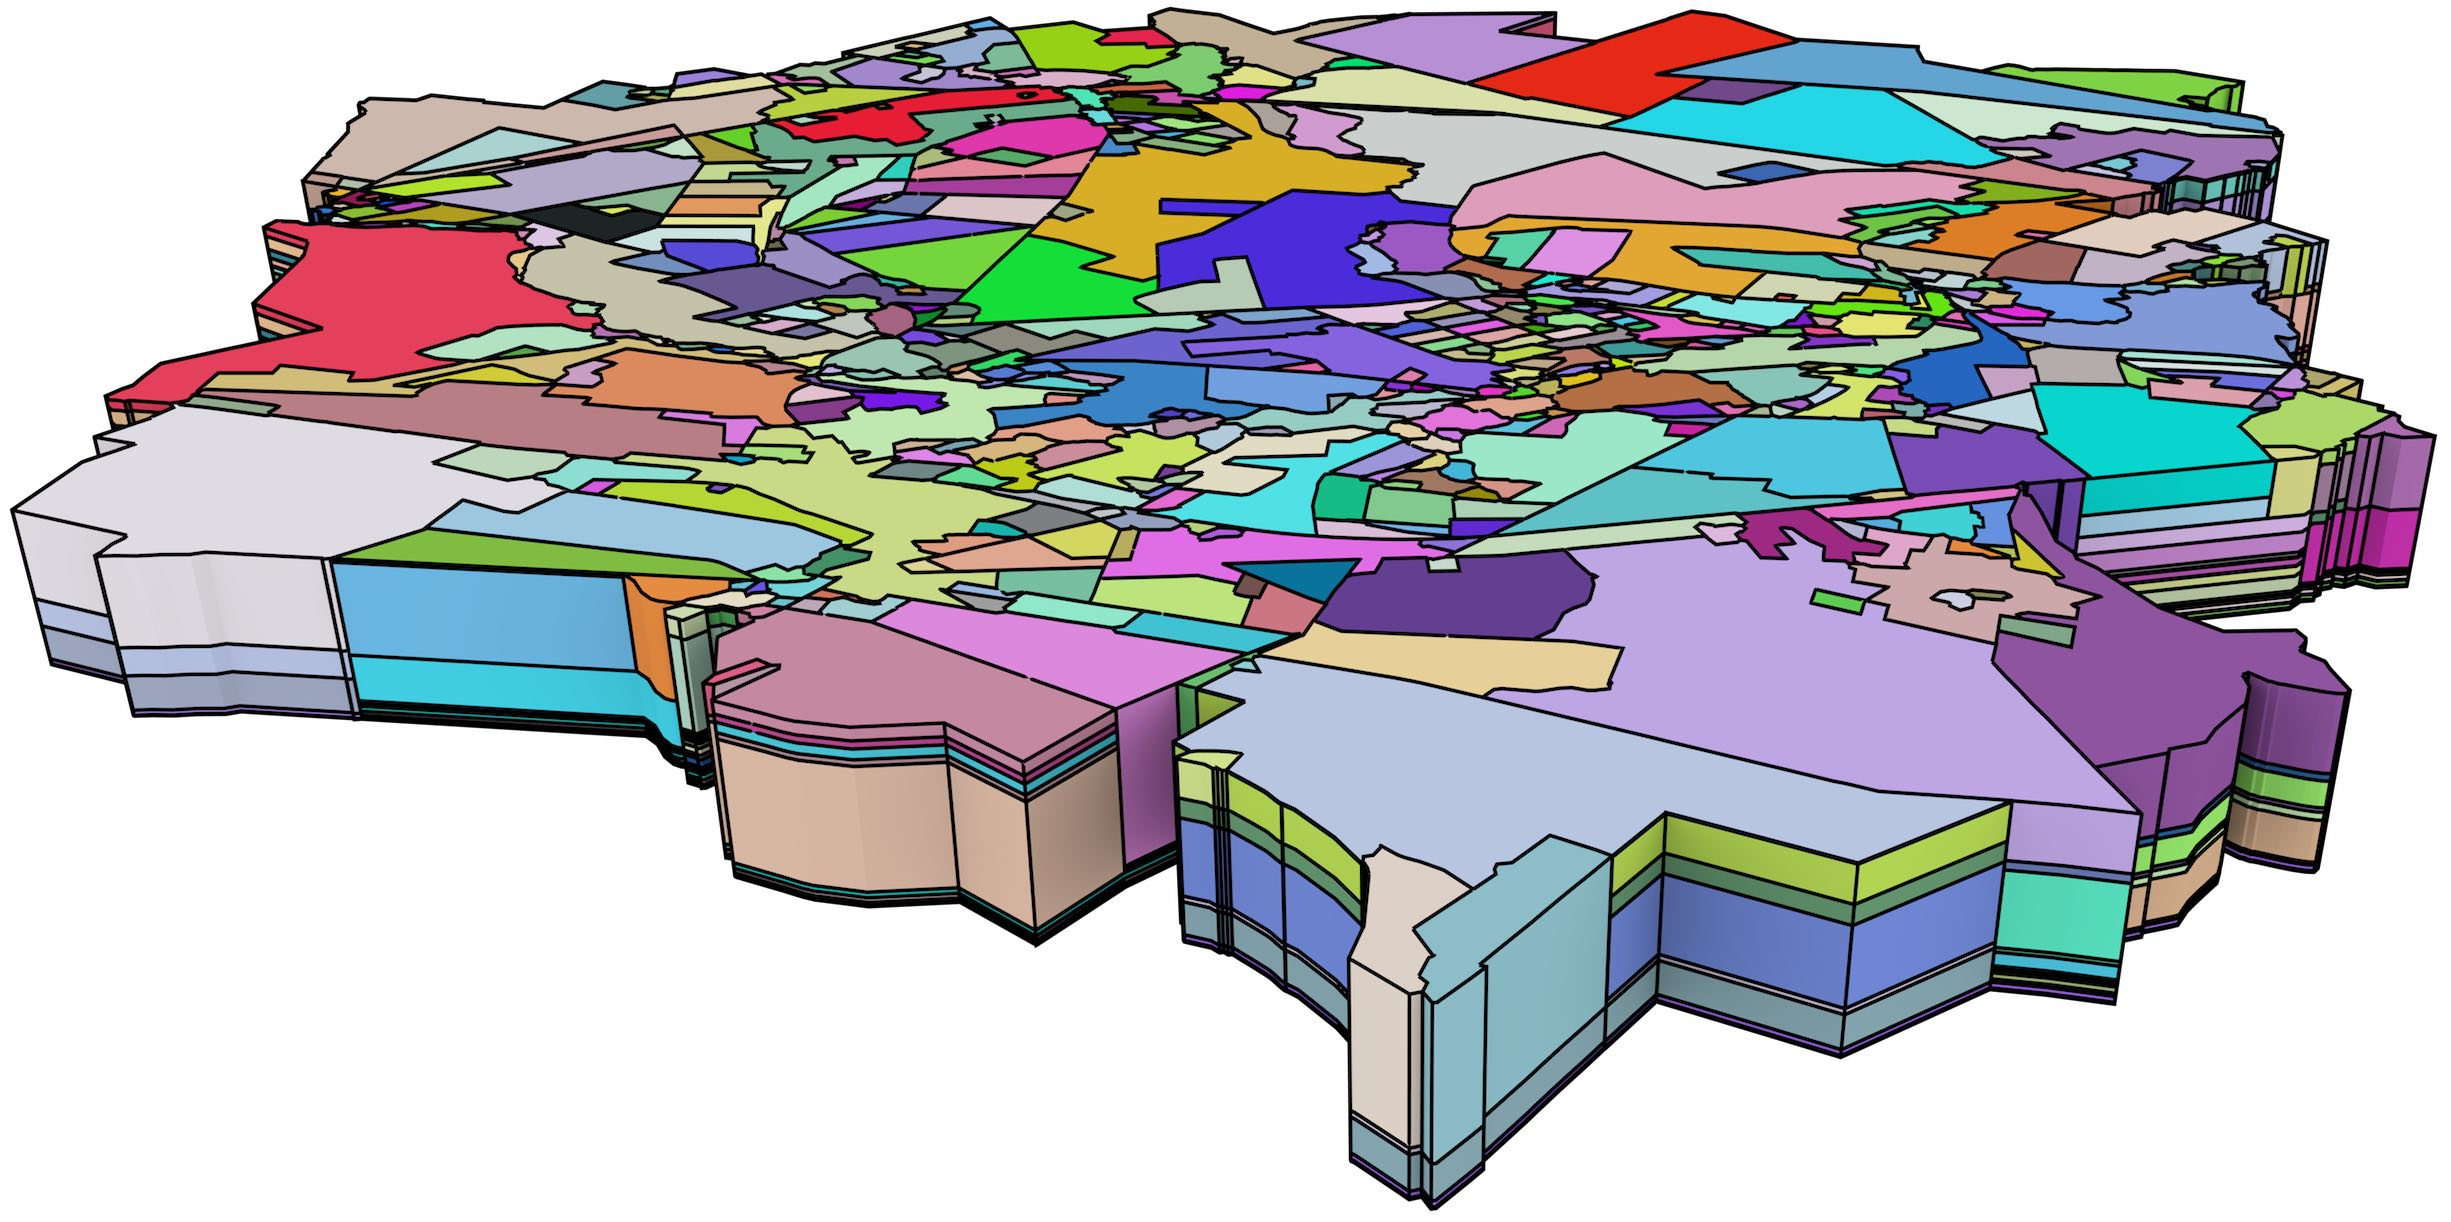
\includegraphics[width=\linewidth]{figs/atkis}
\caption[A large 2D+scale dataset]{A large 2D+scale dataset from \citet{Meijers11}, which uses equally spaced generalisation operations that merge two adjacent polygons.}
\label{fig:atkis}
\end{figure}

In this latter dataset, an additional test was made using its first 250 polyhedra, which lie on the top of \reffig{fig:atkis}, comparing the time used for the construction of vertices, faces and volumes with and without the use of indices.
The results of both methods were equivalent using the approach shown in \refse{se:ndqueries}.
On average, using indices resulted in a faster vertex construction time by a factor of 2 200, faster face construction by a factor of 56 and faster volume construction by a factor of 38.
However, as \reffig{fig:construction-times} shows, these speed gains are not even throughout the 250 polyhedra.
The speed gained from using an index on the vertices increases roughly linearly on the number of constructed vertices, while that gained on from the faces index remains roughly constant between a factor of 50 and 60, and that gained from the volumes index tends to slowly increase as well.
\begin{figure*}[tbp]
\centering
\subfloat[]{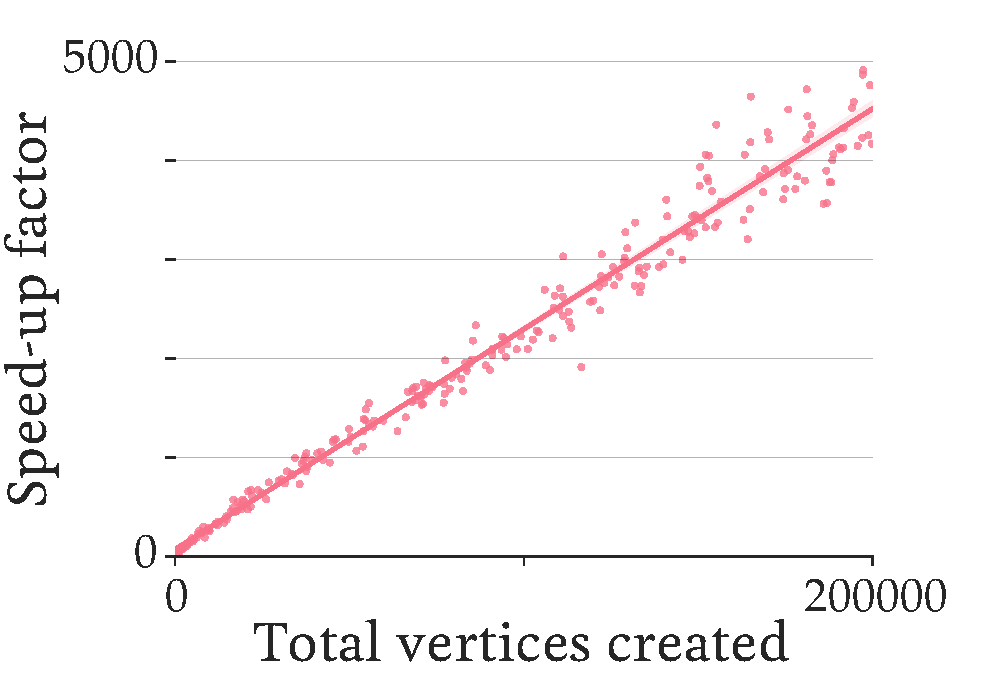
\includegraphics[width=0.33\linewidth]{figs/construction-vertices}\label{subfig:construction-vertices}}
\subfloat[]{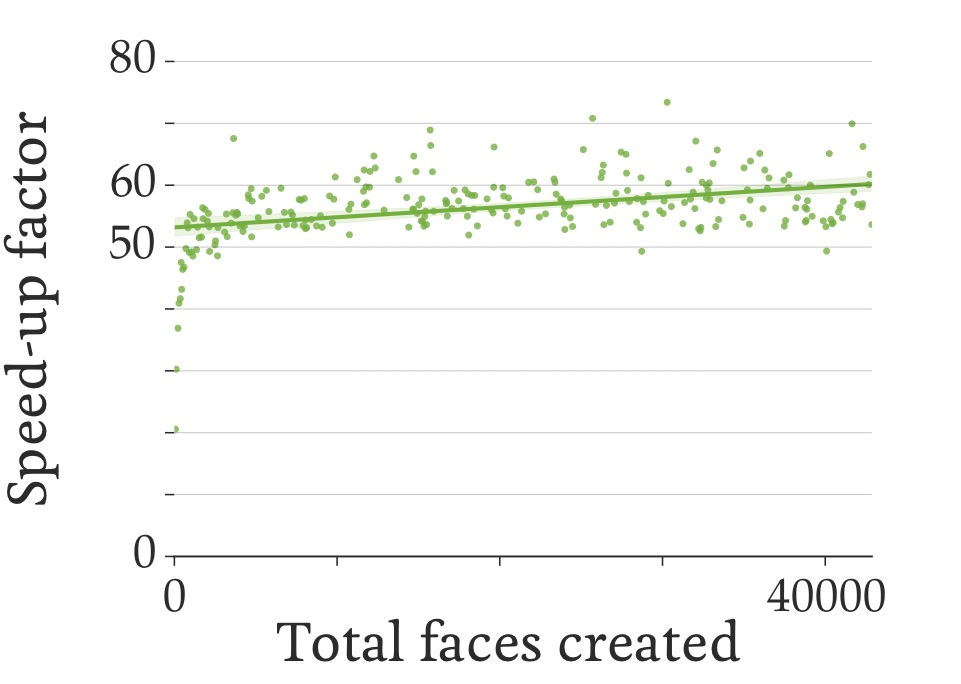
\includegraphics[width=0.33\linewidth]{figs/construction-faces}\label{subfig:construction-faces}}
\subfloat[]{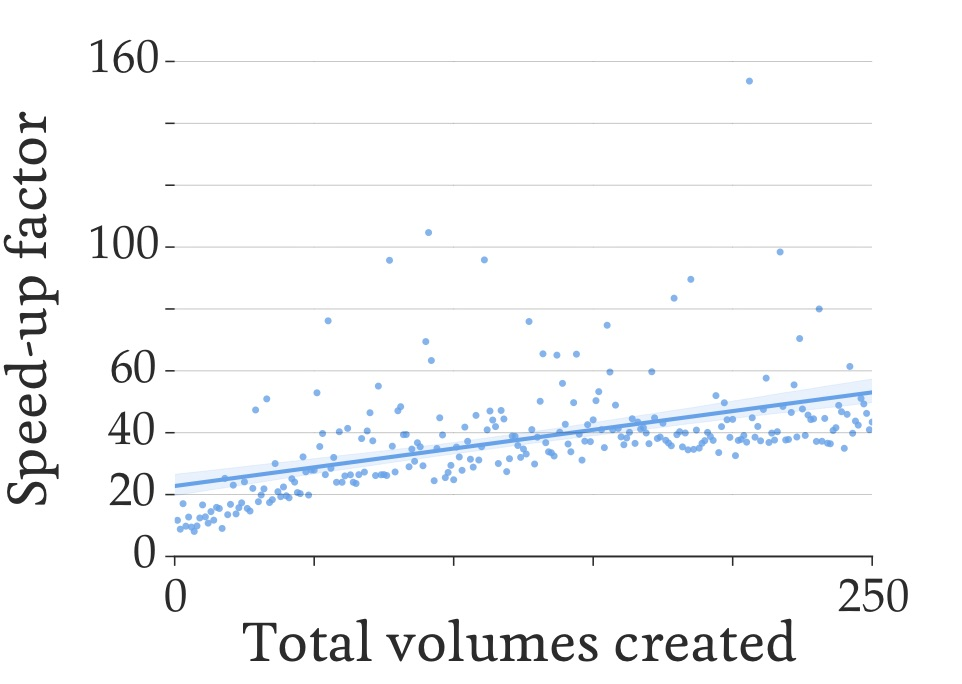
\includegraphics[width=0.33\linewidth]{figs/construction-volumes}\label{subfig:construction-volumes}}
\caption[Construction time speed-up from the use of indices]{Construction time speed-up from the use of indices on the (a) vertices, (b) faces and (c) volumes.}
\label{fig:construction-times}
\end{figure*}

\section{Conclusions}
\label{se:incremental-conclusions}

Creating computer representations of higher-dimensional objects can be complex.
Common construction methods used in 3D, such as directly manipulating combinatorial primitives, or using primitive-level construction operations (\eg\ Euler operators \citep{Mantyla88}), rely on our intuition of 3D geometry, and thus do not work well in higher dimensions.
It is therefore all too easy to create invalid objects, which then cannot be easily interpreted or fixed.

The incremental construction method proposed in this section follows a completely different approach, which has a solid underpinning in the Jordan-Brouwer separation theorem \citep{Lebesgue11,Brouwer11}.
By exploiting the principles of boundary representation, it constructs an $i$-cell based on a set of its bounding $(i-1)$-cells.
Since individual $(i-1)$-cells are easier to describe than the $i$-cell, it thus subdivides a complex representation problem into a set of simpler, more intuitive ones.
The method can moreover be incrementally applied to construct cell complexes of any dimension, starting from a set of vertices in $\mathbb{R}^n$ defined by a $n$-tuple of their coordinates, and continuing with cells of increasing dimension---creating edges from vertices, faces from vertices or edges, volumes from faces and so on.

While a set of $(i-1)$-cells bounding an $i$-cell can be said to already form a complete representation of an $i$-cell, this is not sufficient for its representation in a topological data structure, which requires the topological relationships between the $(i-1)$-cells to be computed.
The incremental construction algorithm proposed in this section thus computes the relationships that are required for two data structures: generalised or combinatorial maps.
However, these relationships are also applicable to most other data structures.

The algorithm is efficient due to its use of indices using the lexicographically smallest vertex of every cell per dimension, as well as an added index using the lexicographically smallest vertex of the bounding ridges of the cell that is being built.
It generates an $i$-cell in $O(d^{2})$ in the worst case, with $d$ the total number of darts in the cell.
However, it fares markedly better in real-world datasets, as cells do not generally share the same lexicographically smallest vertex.
By checking all matching ridges within a cell's facets, the algorithm can optionally verify that the cell being constructed forms a combinatorially valid quasi-manifold, avoiding the construction of invalid configurations.

A publicly available implementation of the algorithm has been made based on CGAL Combinatorial Maps, and its source code has been released under a permissive licence.
It is worth noting that it is one of very few general-purpose object construction methods that has been described and implemented for four- or higher-dimensional cell complexes.

The implementation has been tested with simple 2D--4D objects, as well as with large 2D+scale datasets from \citet{Meijers11}.
The constructed objects were tested to verify that they form valid combinatorial maps.
The small objects were also manually inspected, visualised, and where possible, they were compared with equivalent objects known to be valid using the method discussed in \refse{se:ndqueries}.
